\section{Zielsetzung}
\label{sec:ziel}

Ziel dieses Versuches ist es, Isotope von Vanadium und Silber zu untersuchen und ihre Halbwertszeit zu bestimmen.


\section{Theorie}
\label{sec:Theorie}

Ein Atomkern ist nur dann stabil, wenn seine Neutronenzahl, je nach Nuklid, 20 bis 50\% höher ist, als seine Protonenzahl. Ein Atomkern, der außerhalb
dieses Stabilitätsbereiches liegt, zerfällt dabei in verschiedene Zerfallsprodukte. Bei diesen Zerfallsprodukten handelt es sich wiederum um Atomkerne, die
stabil oder instabil sein können, aber auch um Teilchen wie Neutronen.\\
Wann genau ein instabiler Atomkern zerfallen wird, ist unmöglich zu sagen. Es kann für ein bestimmtes Isotop lediglich eine Halbwertszeit angegeben werden.
Sie gibt dabei die Zeit an, in der die Hälfte einer bestimmten Menge Atomkerne des selben Isotops
zerfallen sein wird. Die Halbwertszeit variiert zwischen unterschiedlichen Atomkernen um bis zu 23 Größenordnungen.


\subsection{Kernreaktionen mit Neutronen}

Da die Halbwertszeit von einigen Atomkernen sehr gering ist, müssen diese erst kurz vor Beginn der Messung der Halbwertszeit hergestellt werden. Um aus stabilen Kernen
instabile zu machen, müssen diese mit Neutronen beschossen werden. Der beschossene Kern nimmt dabei die kinetische Energie des Neurons auf und verteilt diese auf seine
Nukleonen, was ihn in einen angeregten Zustand versetzt. Um aus dem angeregten Zustand in seinen Grundzustand zurückzukehren, emmitiert der Kern ein $\gamma$-Quant. \\
\newline
$\ce{^{m}_zA + ^{1}_0n -> ^{m+1}_zA + \symup{\gamma}}$ \\
\newline
Aufgrund des zusätzlichen Neutrons ist der neue Atomkern allerdings meistens instabil. Er zerfällt deshalb unter Emission eines Elektrons und eines Antineutrinos in einen
stabilen Kern. Die kinetische Energie, die sich Elektron und Antineutrino aufteilen, kommt dabei aus der Massendifferenz zwischen dem instabilen Kern und den
Zerfallsprodukten. \\
\newline
$  \ce{  ^{m+1}_zA -> ^{m+1}_{z+1}C + \symup{\beta}- + E_{Kin} + \bar{\symup{\nu}}_e}   $ \\
\newline
Die Wahrscheinlichkeit, mit der ein stabiler Atomkern ein Neutron aufnimmt, ist vom Wirkungsquerschnitt $\sigma$ abhängig. Dieser gibt hierbei die Fläche an, die ein Kern
besitzen müsste, wenn jedes diese Fläche treffende Neutron eingefangen werden würde. Er wird in $10^{-24} \, \si{\centi\metre\squared} \coloneqq 1 \, \mathrm{barn}$
angegeben und ist durch
\begin{equation}
    \label{eqn:Sigma}
    \sigma = \frac{u}{nKd}
\end{equation}
definiert. Dabei ist $d$ die Dicke, $K$ die Anzahl der Atome pro $\unit{\centi\meter^3}$, $n$ die Anzahl der Neutronen pro Sekunde und $u$ die Anzahl der Einfänge.
Der Wirkungsquerschnitt für den Neutroneneinfang ist zudem stark abhängig von der Geschwindigkeit der Neutronen und
somit dessen kinetischer Energie.


\subsection{Erzeugung niederenergetischer Neutronen}

Da Neutronen alleine eine mittlere Lebensdauer von $\SI{15}{\minute}$ haben, müssen weitere Kernreaktionen verwendet werden, um vor dem Anregen freie Neutronen zu erhalten.
Für diesen Versuch wird die Reaktion \\
\newline
$\ce{^{9}_{4}Be + ^{4}_{2}\symup{\alpha} -> ^{12}_{6}C + ^{1}_0n}$ \\
\newline
verwendet. Die somit gewonnenen Elektronen sind jedoch hochenergetisch, was das Eindringen in einen stabilen Kern erschwert. Um die Neutronen abzubremsen, wird die in
\autoref{fig:therm} zu sehende Apparatur verwendet.

\begin{figure}[H]
    \centering
    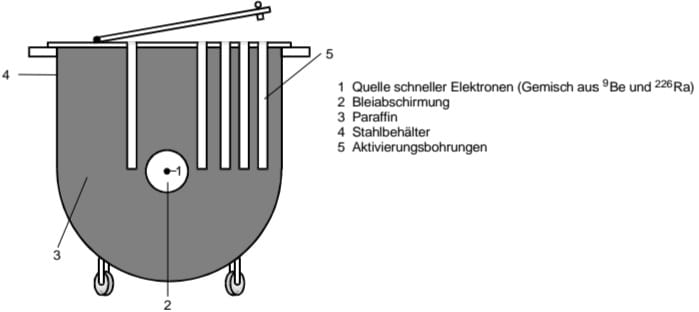
\includegraphics[width=\textwidth]{data/quellethermneutr.jpeg}
    \caption{Querschnitt der verwendeten Quelle für thermische Neutronen.}
    \label{fig:therm}
\end{figure}

In dieser werden die Neutronen durch eine Schicht Paraffin geleitet, bevor sie die anzuregende Probe erreichen. Durch elastische
Stöße mit dem Paraffin verlieren die Neutronen schließlich so viel ihrer Energie, dass diese der mittleren Energie der Moleküle der Umgebung entspricht. Man bezeichnet diese
Neutronen dann als thermische Neutronen.


\subsection{Untersuchung des Zerfalls instabiler Isotope}

Die Zahl $N(t)$ der zum Zeitpunkt $t$ noch vorhandenen Kerne ist durch
\begin{equation}
    \label{eqn:Zerfallsgesetz}
    N(t) = N_0 e^{- \lambda t}
\end{equation}
gegeben, wobei $N_0$ die Zahl der ursprünglich vorhandenen Kerne und $\lambda$ die Zerfallskonstante, die die Wahrscheinlichkeit für einen Zerfall angibt, ist.
Die bereits erwähnte Halbwertszeit, die angibt, nach welcher Zeit die Hälfte aller ursprünglich vorhandenen Kerne zerfallen ist, ist somit auch gegeben als
\begin{equation}
    \label{eqn:T}
    T = \frac{\ln{2}}{\lambda}.
\end{equation}
Durch das Messen von $N(t)$ können also $T$ und $\lambda$ bestimmt werden. Da es jedoch äußerst schwierig ist $N(t)$ direkt zu messen, wird stattdessen die Anzahl an
Zerfällen $N_{\upDelta t}(t)$ in einem Zeitintervall $\upDelta t$ gemessen. Die Größe ist somit definiert durch
\begin{equation*}
    N_{\Delta t}(t) = N(t) - N(t + \Delta t).
\end{equation*}
Dieser Ausdruck lässt sich auch schreiben als
\begin{equation}
    \label{eqn:lnDelta}
    \ln{N_{\Delta t}(t)} = \ln{N_0 (1-e^{- \lambda \Delta t})} - \lambda t,
\end{equation}
woran zu erkennen ist, dass mit Hilfe von Gleichung \eqref{eqn:lnDelta} und einer Ausgleichsrechnung $\lambda$ bestimmt werden kann.
